%%%%%%%%%%%%%%%%%%%%%%%%%%%%%%%%%%%%%%%%%%%%%%%%%%%%%%%%%%%%%%%%%%%%%%%%%%%%%%%%
%% MASTER'S THESIS                                                            %%
%%                                                                            %% 
%% Title (en): Multi-Agent Systems and Organizations                          %%
%% Title (cs): Multiagentní systémy a organizace                              %%
%%                                                                            %%
%% Author: Bc. Lukáš Kúdela                                                   %%
%% Supervisor: Prof. RNDr. Petr Štěpánek, DrSc.                               %%
%%                                                                            %%
%% Academic year: 2011/2012                                                   %%
%%%%%%%%%%%%%%%%%%%%%%%%%%%%%%%%%%%%%%%%%%%%%%%%%%%%%%%%%%%%%%%%%%%%%%%%%%%%%%%%

\section{Dynamic Metamodel}

The dynamic \textit{Thespian} metamodel is used to model dynamic (behavioural) aspects of OCMAS like:
\begin{itemize}
	\item players playing roles within organizations,
	\item players exercising their roles' competences and fulfilling their roles' responsibilities, or
	\item players subscribing to organization events, or
	\item organizations publishing events.
\end{itemize}

%%%%%%%%%%%%%%%%%%%%%%%%%%%%%%%%%%%%%%%%%%%%%%%%%%%%%%%%%%%%%%%%%%%%%%%%%%%%%%%%
\subsection{Player and Organization Interaction}

% Organization protocols
A player and an organization interact through four protocols: \textit{Enact role}, \textit{Deact role}, \textit{Subscribe to event} and \textit{Publish event}.

%%%%%%%%%%%%%%%%%%%%%%%%%%%%%%%%%%%%%%%%%%%%%%%%%%%%%%%%%%%%%%%%%%%%%%%%%%%%%%%%
\subsubsection{Enacting a Role}

% Figure: 'Enact role' protocol
\begin{figure}[ht]
	\centering
	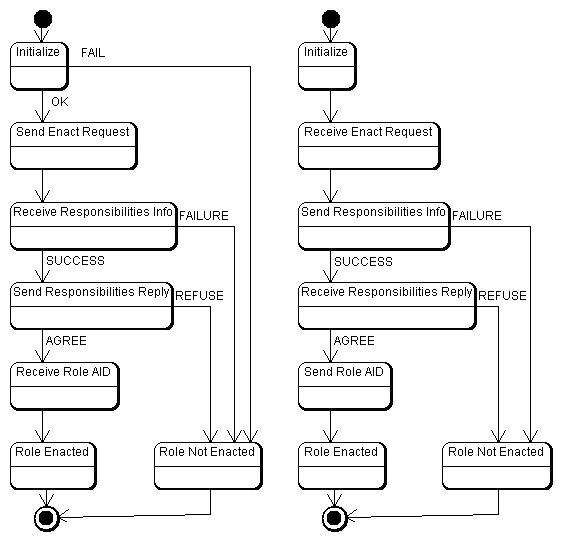
\includegraphics[width=0.8\textwidth]{images/thespian/enact-role-protocol.png}
	\caption{The \textit{Enact role} protocol}
	\label{figure:thespian-enact-role-protocol}
\end{figure}

% 'Enact a role in an organization' - definition
To \textit{enact} a role in an organization means to assume a in an organization.
% Restrictions
Naturally, only a non-enacted or multiple role can be enacted; more precisely, a role can only be enacted in a concrete organization in which it is not already enacted by any player or is defined as a multiple role.
% Protocol
A player who wants to enact a role in an organization, initiates the \textit{Enact role} protocol with that organization.

% 'Enact role' protocol - definition
The \textit{Enact role} protocol consists of the following steps:
\begin{enumerate}
	% 1
	\item The player sends an \textit{Enact role request} message to the organization containing the name of the role it wants to enact.
	% 2	
	\item The organization receives the request message and sends back either
	\begin{itemize}
		% SUCCESS
		\item a \textit{Required Responsibilities} message listing the role's responsibilities if such role exists and can be enacted, i.e. if it is not enacted by any player or is defined as a multiple role, or
		% Failure
		\item a \textit{Failure} message otherwise. 
	\end{itemize}
	% 3	
	\item Upon receiving a \textit{Required Responsibilities} message, the player then determines if it has the required capabilities to fulfil the role's responsibilities and replies either with
	\begin{itemize}
		% AGREE		
		\item an \textit{Agree} message if it has the capabilities, or
		% REFUSE
		\item a \textit{Refuse} message otherwise.
	\end{itemize}
	% 4
	\item Upon receiving an \textit{Agree} message, the organization creates a position and sends a \textit{Role AID} message containing its AID to the player.
	The organization then ends its part in the protocol.
	% 5
	\item The player receives the \textit{Role AID} message and ends its part in the protocol.
\end{enumerate}


%%%%%%%%%%%%%%%%%%%%%%%%%%%%%%%%%%%%%%%%%%%%%%%%%%%%%%%%%%%%%%%%%%%%%%%%%%%%%%%%
\subsubsection{Deacting a Role}

% Figure: 'Deact role' protocol
\begin{figure}[ht]
	\centering
	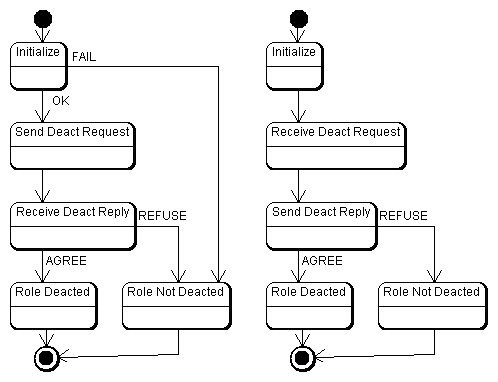
\includegraphics[width=0.8\textwidth]{images/thespian/deact-role-protocol.png}
	\caption{The \textit{Deact role} protocol}
	\label{figure:thespian-deact-role-protocol}
\end{figure}

% 'Deact a role in an organization' - definition
To \textit{deact}\footnote{The word `deact' does not exist in the English language, it is a made-up word.} a role in an organization means to relinquish a role in an organization.
% Restrictions
Naturally, only an enacted and inactive (see section~\ref{section:activating-a-role} for details) role can be deacted; more precisely, a role can only be deacted in a concrete organization in which it is enacted by the player and inactive.
% Protocol
A player who wants to deact a role in an organization, initiates the \textit{Deact role} protocol with that organization.

% 'Deact role' protocol - definition
The following steps comprise the \textit{Deact role} protocol:
\begin{enumerate}
	% 1
	\item The player sends a \textit{Deact role request} message to the organization containing the name of the role it wants to enact.
	% 2	
	\item The organization receives the request message and sends back either
	\begin{itemize}
		% AGREE
		\item an \textit{Agree} message if the role exists and can be deacted, i.e. if it is enacted by the player and inactive, or
		% REFUSE
		\item a \textit{Refuse} message otherwise. 
	\end{itemize}
	The organization then ends its part in the protocol.
	% 3
	\item The player receives the reply message and ends its part in the protocol.
\end{enumerate}

%%%%%%%%%%%%%%%%%%%%%%%%%%%%%%%%%%%%%%%%%%%%%%%%%%%%%%%%%%%%%%%%%%%%%%%%%%%%%%%%
\subsubsection{Subscribing to an Event}

% Figure: 'Subscribe to event' protocol
\begin{figure}[ht]
	\centering
	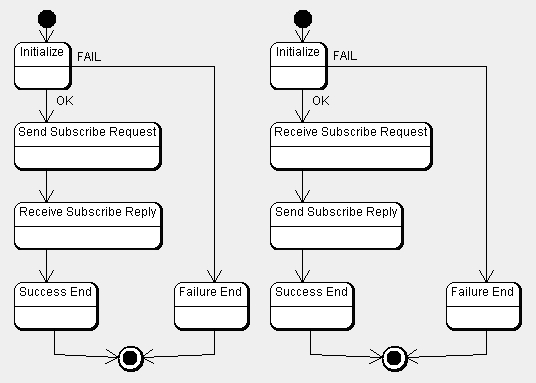
\includegraphics[width=0.8\textwidth]{images/thespian/subscribe-to-event-protocol.png}
	\caption{The \textit{Subscribe to event} protocol}
	\label{figure:thespian-subscribe-to-event-protocol}
\end{figure}

% 'Subscribe to an event in an organization' - definition
Subscribing to an event in an organization means to be notified of an event in an organization.
A player can subscribe to the \textit{role enacted}, \textit{role deacted}, \textit{role activated} and \textit{role deactivated} events raised when a role is enacted, deacted, activated and deactivated respectively.
% Restrictions
Naturally, only an employed player can subscribe to an event; more precisely, an event can only be subscribed to in a concrete organization in which the player enacts a role.
% Protocol
A player who wants subscribe to an event in an organization, initiates the \textit{Subscribe to event} protocol with that organization.

% 'Subscribe to event' protocol - definition
The \textit{Subscribe to event} protocol consists of the following steps:
\begin{enumerate}
	% 1
	\item The player sends a \textit{Subscribe to event request} message containing the name of the role it wants to enact to the organization.
	% 2	
	\item The organization receives the request message and immediately terminates if the message comes from a player that is not employed by that organization.
	If the message comes from a player employed in that organization, it sends back either
	\begin{itemize}
		% AGREE
		\item an \textit{Agree} message if the event exists, or
		% REFUSE
		\item a \textit{Refuse} message otherwise. 
	\end{itemize}
	The organization then ends its part in the protocol.
	% 3
	\item The player receives the reply message and ends its part in the protocol.
\end{enumerate}

%%%%%%%%%%%%%%%%%%%%%%%%%%%%%%%%%%%%%%%%%%%%%%%%%%%%%%%%%%%%%%%%%%%%%%%%%%%%%%%%
\subsubsection{Publishing an Event}

% Figure: 'Publish event' protocol
\begin{figure}[ht]
	\centering
	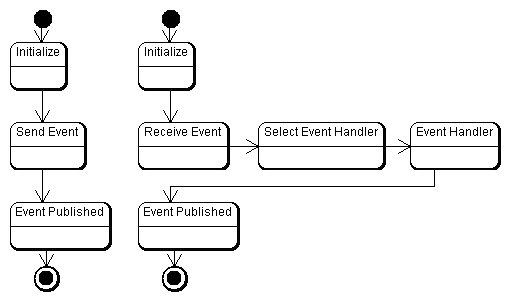
\includegraphics[width=0.8\textwidth]{images/thespian/publish-event-protocol.png}
	\caption{The \textit{Publish event} protocol}
	\label{figure:thespian-publish-event-protocol}
\end{figure}

% 'Publishing an event to subscribed players' - definition
To publish an event to its subscribers means to notify the players subscribed to an event of that event occurring.
% Restrictions
% - none
% Protocol
An organization that wants publish an event to its subscribers, initiates the \textit{Publish event} protocol with the event subscribers.

% 'Publish event' protocol - definition
The following steps comprise the \textit{Publish event} protocol:
\begin{enumerate}
	% 1	
	\item The organization sends an \textit{Event} message containing the name of the event and its argument to the event subscribers.
	The organization then ends its part in the protocol.
	% 2
	\item A subscriber receives the message and handles the event.
	The subscriber then ends its part in the protocol.
\end{enumerate}

%%%%%%%%%%%%%%%%%%%%%%%%%%%%%%%%%%%%%%%%%%%%%%%%%%%%%%%%%%%%%%%%%%%%%%%%%%%%%%%%
\subsection{Player and Role Interaction}

% Role protocols
A player and a role interact via four protocols: \textit{Activate role}, \textit{Deactivate role}, \textit{Invoke competence} and \textit{Invoke responsibility}.

%%%%%%%%%%%%%%%%%%%%%%%%%%%%%%%%%%%%%%%%%%%%%%%%%%%%%%%%%%%%%%%%%%%%%%%%%%%%%%%%
\subsubsection{Activating a Role}
\label{section:activating-a-role}

% Figure: 'Activate role' protocol
\begin{figure}[ht]
	\centering
	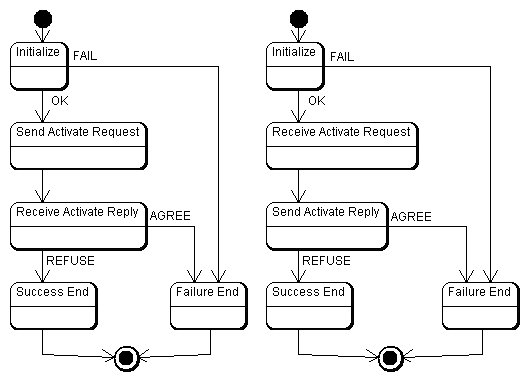
\includegraphics[width=0.8\textwidth]{images/thespian/activate-role-protocol.png}
	\caption{The \textit{Activate role} protocol}
	\label{figure:thespian-activate-role-protocol}
\end{figure}

% 'Activate a role' - definition
To \textit{activate} a role\footnote{More precisely, what is activated is a position---a concrete instantiation of a role in a specific organization enacted by the activating player.} means to begin playing a role, i.e. start exercising its competences and fulfilling its responsibilities.
% Restrictions
Naturally, only an enacted and inactive role can be activated; more precisely, a role can only be activated in a concrete organization in which it is already enacted by the player and inactive.
Furthermore, a player may activate only one role (in all concrete organizations) at a time.
% Protocol
A player who wants to activate a role, initiates the \textit{Activate role} protocol with that role.

% 'Activate role' protocol - definition
The \textit{Activate role} protocol consists of the following steps:
\begin{enumerate}
	% 1
	\item The player sends a \textit{Activate role} request message to the role.
	% 2	
	\item The role receives the request message and immediately terminates if the message comes from anyone else than its player.
	If the message comes from its enacting player, it sends back either
	\begin{itemize}
		% AGREE
		\item an \textit{Agree} message if the role can be activated, i.e. it is inactive, and the player does not have any other active role in the role's organization.
		% REFUSE
		\item a \textit{Refuse} message otherwise. 
	\end{itemize}
	The role then ends its part in the protocol.
	% 3
	\item The player receives the reply message and ends its part in the protocol.
\end{enumerate}

%%%%%%%%%%%%%%%%%%%%%%%%%%%%%%%%%%%%%%%%%%%%%%%%%%%%%%%%%%%%%%%%%%%%%%%%%%%%%%%%
\subsubsection{Deactivating a Role}

% Figure: 'Deactivate role' protocol
\begin{figure}[ht]
	\centering
	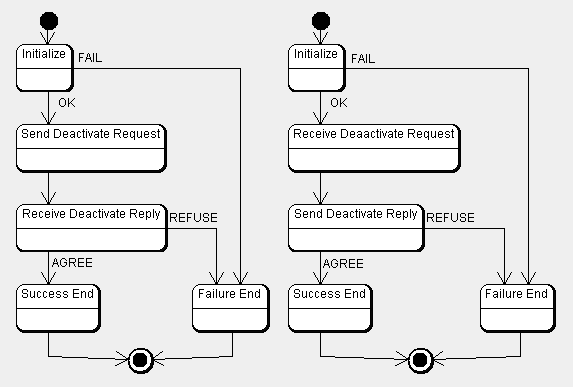
\includegraphics[width=0.8\textwidth]{images/thespian/deactivate-role-protocol.png}
	\caption{The \textit{Deactivate role} protocol}
	\label{figure:thespian-deactivate-role-protocol}
\end{figure}

% 'Deactivating a role' - definition
To \textit{deactivate} a role (more precisely, a position) means to stop playing a role, i.e. stop exercising its competences and fulfilling its responsibilities.
% Restrictions
Naturally, only an enacted and active role can be deactivated; more precisely, a role can only be deacted in a concrete organization in which it is enacted by the player and active.
% Protocol
A player who wants to deactivate a role, initiates the \textit{Deactivate role} protocol with that role.

% 'Deactiavte role' protocol - definition
The following steps comprise the \textit{Deactivate role} protocol:
\begin{enumerate}
	% 1
	\item The player sends a \textit{Deactivate role} request message to the role.
	% 2	
	\item The role receives the request message and immediately terminates if the message comes from anyone else than its player.
	If the message comes its enacting player, it sends back either
	\begin{itemize}
		% AGREE
		\item an \textit{Agree} message if the role can be deactivated, i.e. it is active, or
		% REFUSE
		\item a \textit{Refuse} message otherwise. 
	\end{itemize}
	The role then ends its part in the protocol.
	% 3
	\item The player receives the reply message and ends its part in the protocol.
\end{enumerate}

%%%%%%%%%%%%%%%%%%%%%%%%%%%%%%%%%%%%%%%%%%%%%%%%%%%%%%%%%%%%%%%%%%%%%%%%%%%%%%%%
\subsubsection{Invoking a Competence}

% Figure: 'Invoke competence' protocol
\begin{figure}[ht]
	\centering
	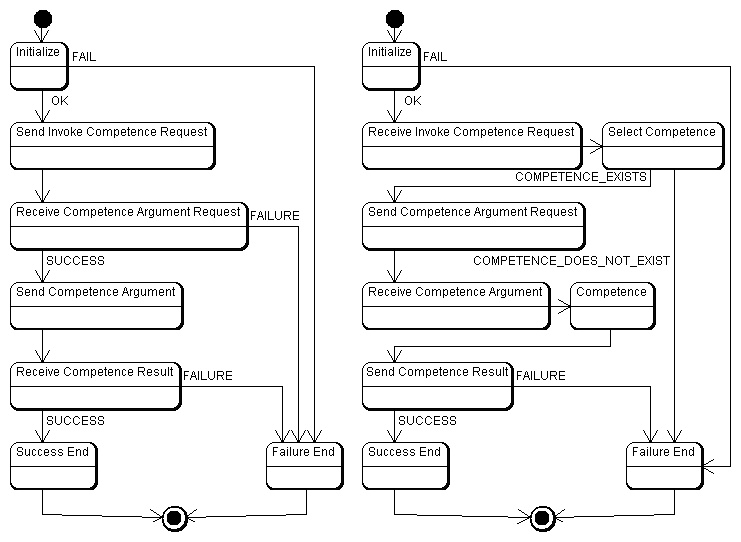
\includegraphics[width=0.8\textwidth]{images/thespian/invoke-competence-protocol.png}
	\caption{The \textit{Invoke competence} protocol}
	\label{figure:thespian-invoke-competence-protocol}
\end{figure}

% 'Invoke a competence on a role' - definition
Invoking a competence on a role (more precisely, a position) happens when a player calls upon its active role to exercise a competence.
% Restrictions
Note that a competence can only be invoked on an active role.
% Protocol
A player who wants to invoke a competence on a role, initiates the \textit{Invoke competence} protocol with that role.

% 'Invoke competence' protocol - definition
The \textit{Invoke competence} protocol consists of the following steps:
\begin{enumerate}
	% 1	
	\item The player sends an \textit{Invoke competence request} request to the role containing the name of the competence to invoke.
	% 2
	\item The role receives the request message and immediately terminates if the message comes from anyone else than its player or it is not active.
	If, on the other hand, the message comes from its player and it is active, it sends back 
	\begin{itemize}
		% SUCCES		
		\item a \textit{Competence argument request} message asking the player to provide the competence argument if the competence exists, or
		% FAILURE
		\item a \textit{Failure} message otherwise. 
	\end{itemize}
	% 3	
	\item Upon receiving the \textit{Competence argument request} message, the player sends the \textit{Competence argument} message carrying the competence argument.
	% 4
	\item The role receives the competence argument and executes the competence and sends back either
	\begin{itemize}
		% SUCCESS
		\item either a \textit{Competence result} message carrying the competence result in case the competence executed successfully, or
		\item a \textit{Failure} message otherwise.
	\end{itemize}
	The role then ends its part in the protocol.
	% 5
	\item The player receives the reply message and ends its part in the protocol.
\end{enumerate}

%%%%%%%%%%%%%%%%%%%%%%%%%%%%%%%%%%%%%%%%%%%%%%%%%%%%%%%%%%%%%%%%%%%%%%%%%%%%%%%%
\subsubsection{Invoking a Responsibility}

% Figure: 'Invoke responsibility' protocol
\begin{figure}[ht]
	\centering
	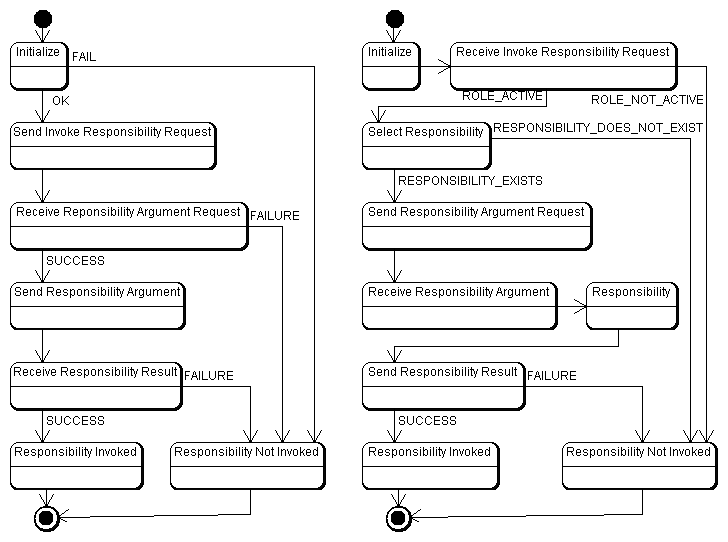
\includegraphics[width=0.8\textwidth]{images/thespian/invoke-responsibility-protocol.png}
	\caption{The \textit{Invoke responsibility} protocol}
	\label{figure:thespian-invoke-responsibility-protocol}
\end{figure}

% 'Invoke a responsibility on a player' - definition
Invoke a responsibility on a player happens when a role (more precisely, a position) calls upon its player to fulfil a responsibility.
% Restrictions
Note that a responsibility can only be invoked by an active role.
% Protocol
A role who wants to invoke a responsibility on its player, initiates the \textit{Invoke responsibility} protocol with its player.

% 'Invoke responsibility' protocol - definition
The following steps comprise the \textit{Invoke responsibility} protocol:
\begin{enumerate}
	% 1	
	\item The role sends an \textit{Invoke responsibility request} request to the role containing the name of the responsibility to invoke.
	% 2
	\item The player receives the request message and immediately terminates if the message comes from anyone else than its active role.
	If, on the other hand, the message comes from its active role, it sends back 
	\begin{itemize}
		% SUCCES		
		\item a \textit{Responsibility argument request} message asking the role to provide the responsibility argument if the responsibility exists, or
		% FAILURE
		\item a \textit{Failure} message otherwise. 
	\end{itemize}
	% 3	
	\item Upon receiving the \textit{Responsibility argument request} message, the role sends the \textit{Responsibility argument} message carrying the responsibility argument.
	% 4
	\item The player receives the responsibility argument and executes the responsibility and sends back either
	\begin{itemize}
		% SUCCESS
		\item a \textit{Responsibility result} message carrying the responsibility result in case the responsibility executed successfully, or
		\item a \textit{Failure} message otherwise.
	\end{itemize}
	The player then ends its part in the protocol.
	% 5
	\item The role receives the reply message and ends its part in the protocol.
\end{enumerate}